\section{Results}
\label{Resul}

The following Section summarises the work by presenting the obtained results. Comments on the goodness of such results are also present, together with possible future developments. 
The popularity distribution computed through Eq. (\ref{Popc}) shows a gaussian-like distribution centred in 0 (Fig. \ref{PopDist}), meaning that on average comments are neutral, with lateral tails of comments with strong polarity, both positive and negative. Recommendations play a small role, because of some outliers causing the normalised recommendation count to be quite a small number. It is fundamental for this distribution to be unbiased as it will be used to estimate controversy in different articles. 

\begin{figure}
\centering
\begin{subfigure}{0.45\tw}
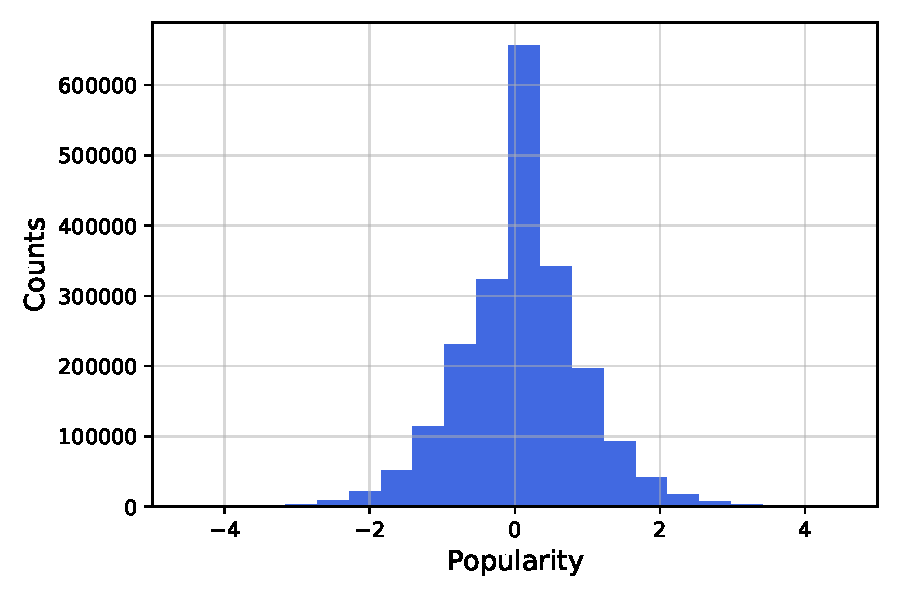
\includegraphics[width=\tw]{Pictures/PopularityDist.pdf}
\caption{Popularity distribution for comments.}
\label{PopDist}
\end{subfigure}

\begin{subfigure}{0.45\tw}
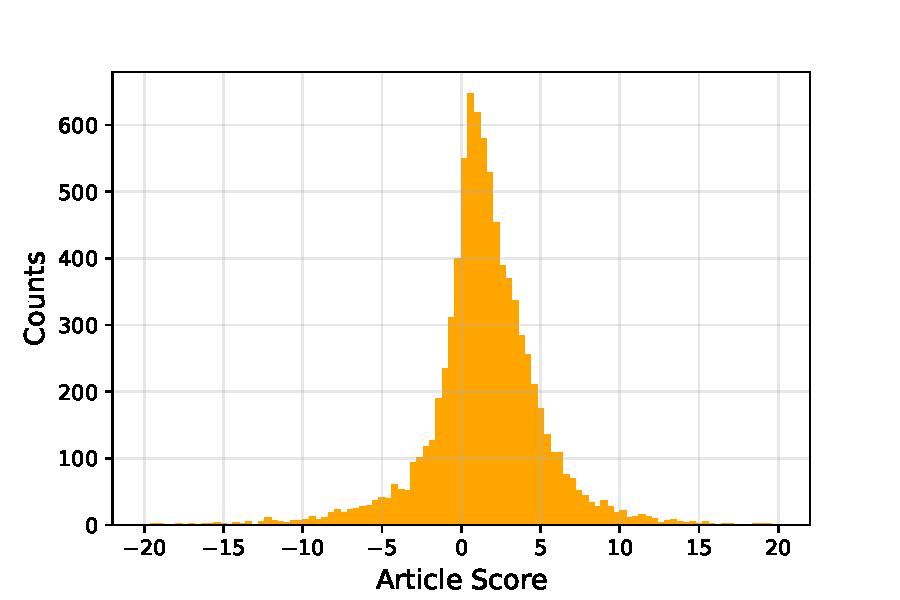
\includegraphics[width=\tw]{Pictures/articleScoreDist.pdf}
\caption{Popularity distribution for comments.}
\label{PopDist}
\end{subfigure}
\end{figure}

The article score distribution shows a similar behaviour; it is reported in Fig. \ref{AScore} even though it will not be included in further analyses. Again, the article Score calculated with Eq. \ref{ASeq} show a quite symmetrical distribution, meaning that the